% *********************************************************************
% © 2021–2024 Jeremy Sylvestre
%
% Permission is granted to copy, distribute and/or modify this document
% under the terms of the GNU Free Documentation License, Version 1.3 or
% any later version published by the Free Software Foundation; with no
% Invariant Sections, no Front-Cover Texts, and no Back-Cover Texts. A
% copy of the license is included in the appendix entitled “GNU Free
% Documentation License” that appears in the output document of this
% PreTeXt source code. All trademarks™ are the registered® marks of
% their respective owners.
%
% *********************************************************************

\newcommand*{\xmin}{0}
\newcommand*{\xmax}{10}
\newcommand*{\ymin}{-3}
\newcommand*{\ymax}{4}

%
% DE is y' = (y + 1) (y - 2)
%
% Solutions are
%   y = (2 + A e^{3t}) / (1 - A e^{3t})
% where
%   A = (y0 - 2) / (y0 + 1)
% BUT
% h.scaling solutions by 10

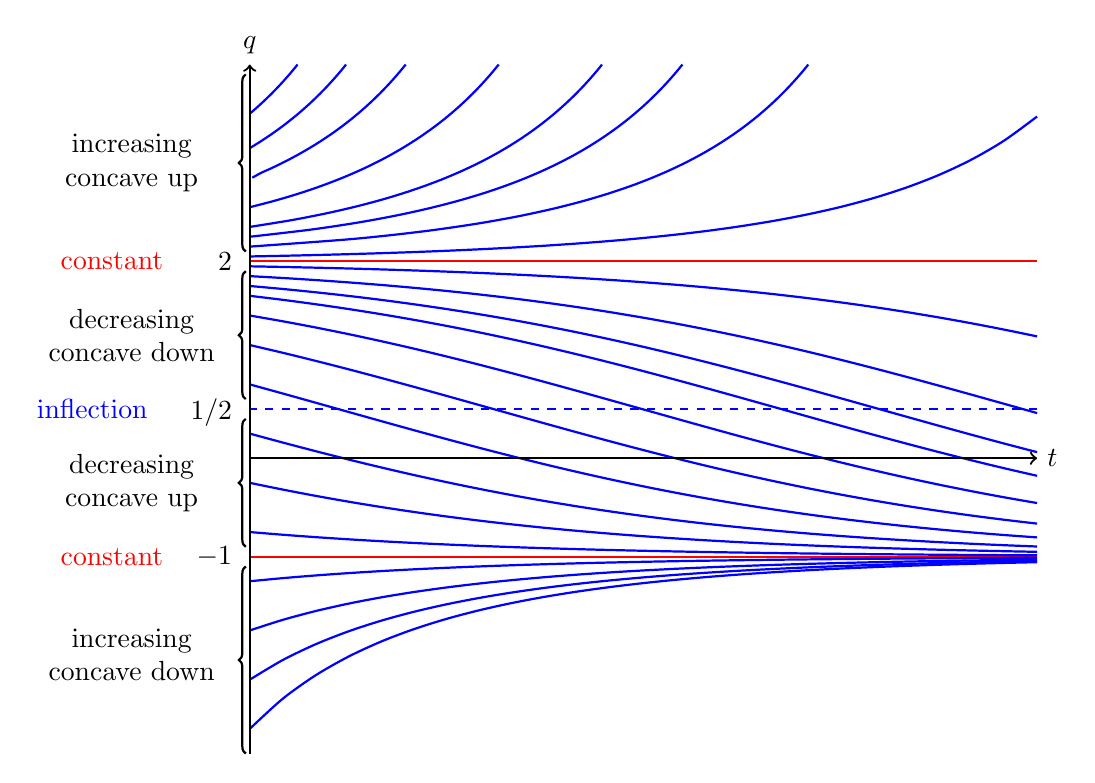
\begin{tikzpicture}
[
	closedpt/.style={circle,draw,fill,inner sep=0pt,minimum size=4pt},
	openpt/.style={circle,draw,inner sep=0pt,minimum size=4pt},
	yscale=1.25
]

	\foreach \q in {-1,2} {
		\draw[red,thick] (\xmax,\q) -- (\xmin,\q);
		\node[left,xshift=-0.1cm] at (0,\q) {$\q$};
		\node[red,xshift=-1.75cm] at (0,\q) {constant};
	}

	\draw[dashed,blue] (\xmax,0.5) -- (\xmin,0.5);
	\node[left,xshift=-0.1cm,yshift=-0.05cm] at (0,0.5) {$1/2$};
	\node[blue,xshift=-2cm] at (0,0.5) {inflection};

	\draw[thick, decorate, decoration = {brace}, xshift=-0.05cm]  (0,\ymin) -- (0,-1.1);
	\node[align=center,xshift=-1.5cm] at (0,-2) {increasing \\ concave down};

	\draw[thick, decorate, decoration = {brace}, xshift=-0.05cm] (0,-0.9) -- (0,0.4);
	\node[align=center,xshift=-1.5cm] at (0,-0.25) {decreasing \\ concave up};

	\draw[thick, decorate, decoration = {brace}, xshift=-0.05cm] (0,0.6) -- (0,1.9);
	\node[align=center,xshift=-1.5cm] at (0,1.25) {decreasing \\ concave down};

	\draw[thick, decorate, decoration = {brace}, xshift=-0.05cm] (0,2.1) -- (0,3.9);
	\node[align=center,xshift=-1.5cm] at (0,3) {increasing \\ concave up};

	\foreach \q in {-2.75,-2.25,-1.75,-1.25,-0.75,-0.25,0.25,0.75,1.15,1.45,1.65,1.75,1.85,1.95,2.05} {
		\pgfmathparse{ (\q - 2) / (\q + 1) }\edef\Acoeff{\pgfmathresult}%
		\draw[thick,blue,smooth,domain=0:\xmax] plot (\x, { (2 + \Acoeff * exp(3 * \x / 10)) / (1 - \Acoeff * exp(3 * \x / 10)) });
	}

	% above q=2 these are exponential functions and things explode,
	% so we invert and plot as a function t = ...
	% in order to be able to specify range instead of domain
	\foreach \q in {2.15,2.25,2.35,2.55,2.85,3.15,3.5} {
		\pgfmathparse{ (\q + 1) / (\q - 2) }\edef\Acoeff{\pgfmathresult}%
		\draw[thick,blue,smooth,domain=\q:\ymax] plot ({ 10 * ln(\Acoeff * (\x - 2) / (\x + 1)) / 3 }, \x);
	}

	% axes
	\draw[->,thick] (\xmin,0) -- (\xmax,0) node[right] {$t$};
	\draw[->,thick] (0,\ymin) -- (0,\ymax) node[above] {$q$};

\end{tikzpicture}
